\section {Estudo de Caso}

Visando a validação da solução apresentada na Seção \ref{sec:solucao}, procurou-se aplicar em estudo de caso em umas das instuições citadas pelo Acórdão no 2314/2013 \cite{TCU:2013}. Dentre estas, O Instituto do Patrimônio Histórico e Artístico Nacional que é autarquia federal responsável pela gestão de diversos processos de preservação do patrimônio cultural, permitiu o acesso ao código-fonte Sistema Integrado de Gestão do Conhecimento (SICG), que foi desenvolvido por contrato de terceirização com princípios ágeis, Lean e Kanban, a fim de avaliar a qualidade interna do produto. 

O Sistema Integrado de Gestão do Conhecimento (SICG) teve como objetivo automatizar o processo de trabalho decorrente da metodologia de inventário, cadastro, normatização, fiscalização, planejamento e análise e gestão do patrimônio material. Esta solução de software foi construído na linguagem Java com a utilização de\textit{frameworks} conhecidos no mercado, como por exemplom VRaptor e Hibernate, durante 24 \textit{releases} mensais.

\subsection{Protocolo do Estudo de Caso}
Seguindo a metodologia proposta por Wohlin \cite{wohlin2012experimentation}, foi construído um protocolo de estudo de caso que foi baseado em Brereton \cite{brereton2008using} quanto aos aspectos gerais e Yin \cite{yin2011applications} com relação as ameaças à validade do estudo. 

O Objeto do Estudo de Caso é a avaliação dos Cenários de Limpeza de código-fonte em ambiente de \textit{data warehousing} a fim de verificar a qualidade interna do produto. no qual a fonte de coleta dos dados é o código-Fonte do Sistema Integrado de Gestão do Conhecimento.

Com relação as ameaças citadas por Yin, a validade de construção ao se definir objetivos com evidências diferentes (Taxa de Aproveitamento de Oportunidades e Cenários de Limpeza de Código-Fonte). Com relação a validade interna do estudo está garantida quando se consegue avaliar em níveis diferentes ou fontes de informação diferentes (projeto e classe) resultados semelhantes.Quanto a validade externa, destaca-se que a utilização de um estudo de caso não é suficiente para generalizar os resultados dele obtidos, sendo necessário a utilização de estudo em múltiplos casos, a fim de comprovar resultados genéricos \cite{yin2011applications}. Com relação a confiabilidade, a partir da documentação da implementação do ambiente de \textit{Data Warehousing} conjuntamente com o protocolo de estudo de caso e as bases de dados das métricas de código-fonte, garante-se a repetição do estudo de caso e por conseguinte a confiabilidade.




\subsection{Execução e Resultados do Estudo de Caso}
\label{sec:resultados}
Para analisar os cenários de limpeza de código-fonte, foram extraídas as métricas de código-fonte de cada classe e analisadas conforme a Tabela \ref{tab:cenarios}. Para cada \textit{release}, foram identificados cenários de limpeza de código-fonte conforme a Figura \ref{fig:cenarios-release}.


\begin{figure}[ht!]
\centering
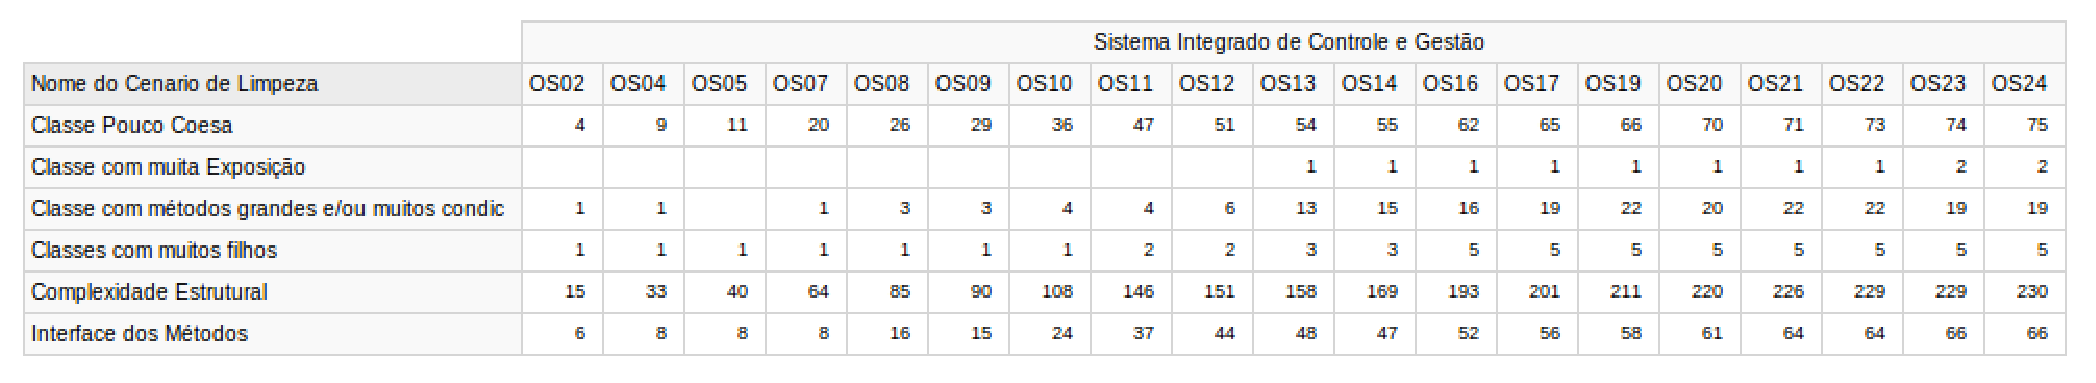
\includegraphics[keepaspectratio=true,scale=0.43]{figuras/total-cenario-tipo.eps}
\caption{Total de Cenários de Limpeza de Código-Fonte identificados por cenário e \textit{Release}}
\label{fig:cenarios-release}
\end{figure}
\FloatBarrier


Realizando uma consulta OLAP de consolidação, obteve-se o número total de cenários de limpeza por cada uma das releases de software analisadas tal como se observa na Figura \ref{fig:cenarios-total}.

\begin{figure}[ht!]
\centering
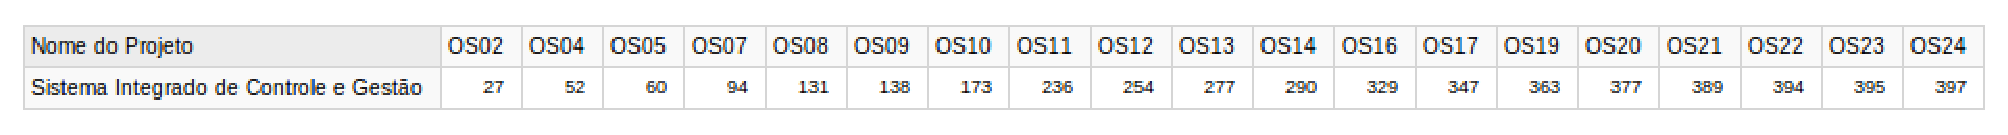
\includegraphics[keepaspectratio=true,scale=0.45]{figuras/total-cenarios-release.eps}
\caption{Total de Cenários de Limpeza de Código-Fonte por Release}
\label{fig:cenarios-total}
\end{figure}
\FloatBarrier

Conforme é possível observar nas Figuras \ref{fig:cenarios-release} e \ref{fig:cenarios-total}, foram detectados mais cenários de limpeza de código-fonte dos tipos \textbf{Complexidade Estrutural}, \textbf{Classe Pouco Coesa} e \textbf{Interface dos Métodos} respectivamente. Os três Cenários de Limpeza com menor número de incidências foram \textbf{Classe com Muita Exposição}, \textbf{Classe com Muitos Filhos} e \textbf{Classe com Métodos Muito Grande e/ou com muitos condicionais}.

Em uma escala de priorização, de qual cenário de limpeza de código-fonte deve ser tratado primeiro, recomenda-se, para o projeto analisado, tratar o cenário de \textbf{Complexidade Estrutural}, pois este sozinho chega a responder entre 55\% a 68\% da quantidade total de cenários identificados. Além da identificação dos cenários de limpeza de código-fonte no projeto como todo, identificou-se, como se mostra na Figura \ref{fig:worst-10-cenarios}, as 10 classes que apresentaram a maior quantidade de cenários de limpeza.


\begin{figure}[ht!]
\centering
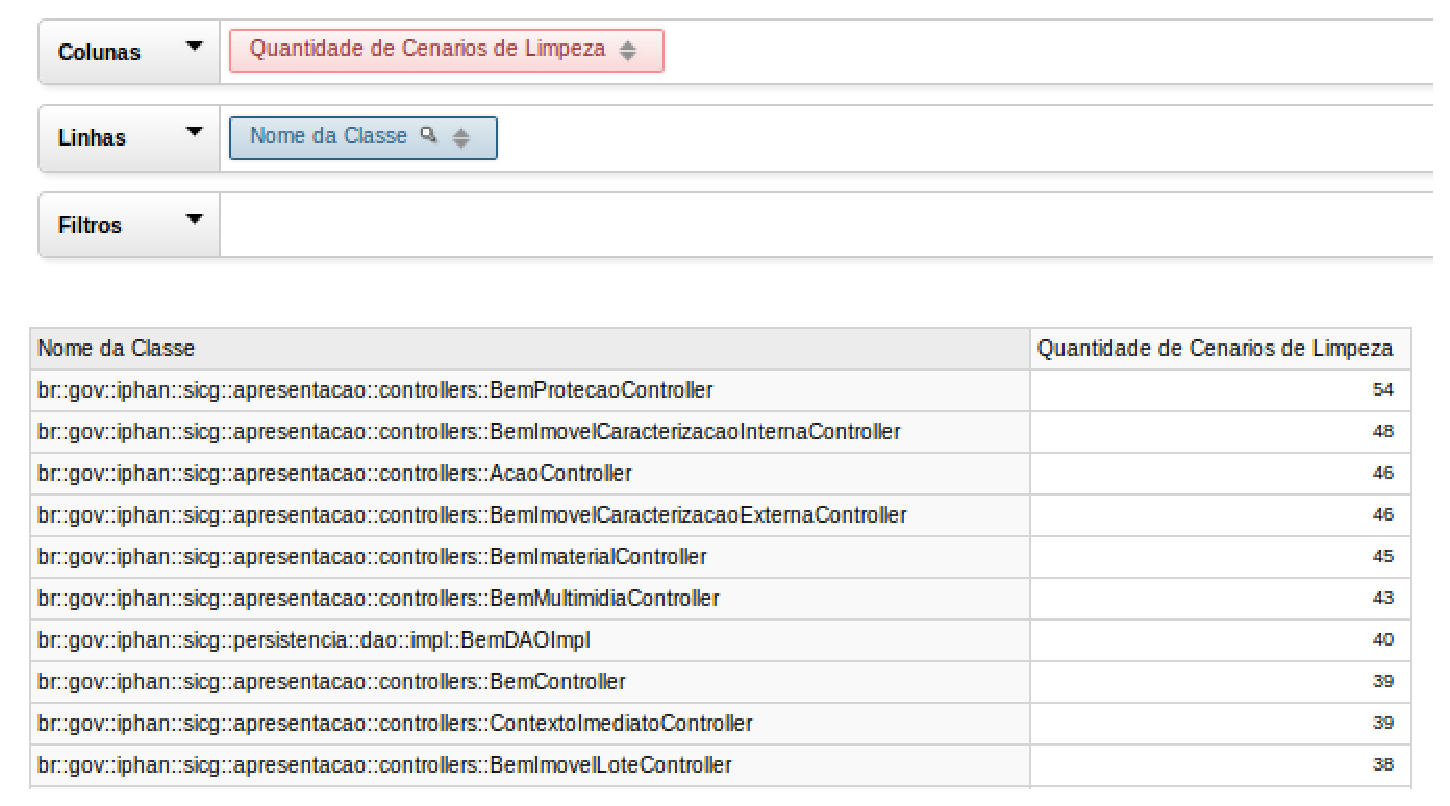
\includegraphics[keepaspectratio=true,scale=0.55]{figuras/10-best.eps}
\caption{As 10 classes com maior número de Cénarios de Limpeza}
\label{fig:worst-10-cenarios}
\end{figure}
\FloatBarrier

Com o número de classes e os cenários de limpeza de código-fonte, foi possível calcular a Taxa de Aproveitamento de Oportunidade de Melhoria de Código-Fonte por cada release do software conforme se mostra na Figura \ref{fig:taxa-cenarios}.

\begin{figure}[H]
\centering
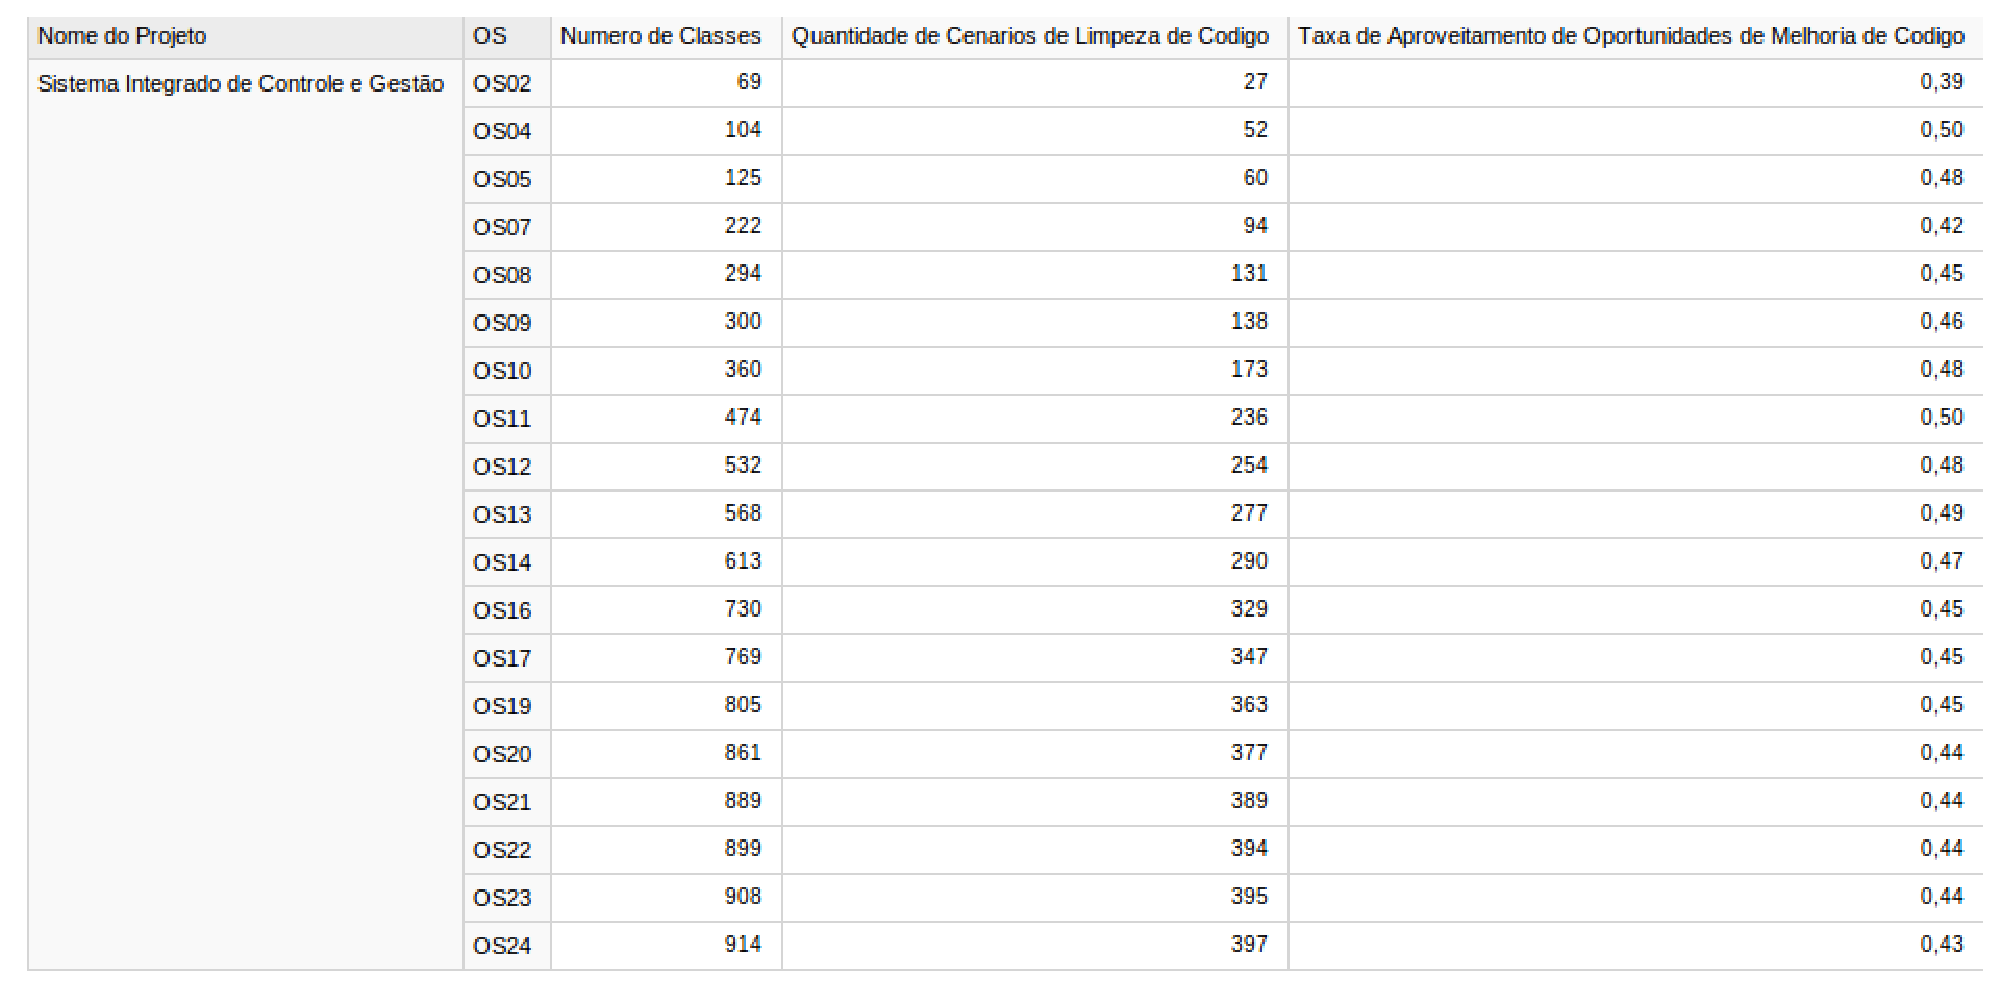
\includegraphics[keepaspectratio=true,scale=0.38]{figuras/taxa-parcial.eps}
\caption{Taxa de Aproveitamento de Oportunidades de Melhoria de Código-Fonte}
\label{fig:taxa-cenarios}
\end{figure}
\FloatBarrier

Observa-se, por meio da Figura \ref{fig:taxa-cenarios}, que o valor da Taxa de Aproveitamento de Oportunidade de Melhoria de Código-Fonte possui uma tendência entre 0,4 a 0,5. Este fato pode indicar duas hipóteses: a primeira de que o projeto cresceu em uma taxa muito maior que a quantidade de cenários de limpeza, indicando assim uma estabilidade na complexidade do projeto; ou que não foram promovidas atividades de melhoria de código-fonte ao longo das 24 releases.
